\subsection{QUY TẮC ĐẾM}
%-------------Trắc nghiệm nhiều lựa chọn
\ind{PHẦN I.} \inden{Câu trắc nghiệm nhiều phương án lựa chọn. Mỗi câu hỏi học sinh chỉ chọn một phương án.}
\setcounter{ex}{0}
\Opensolutionfile{ans}[ans/ans-c1b1-lc]
%Câu 1
\begin{ex}%[0D8N1-1]%[Biên soạn tài liệu dạy học bộ KNTT-CS]%[GV Lien Nguyen]
	Một trong một cửa hàng bán kem có $6$ loại kem que và $3$ loại kem ốc quế. Có bao nhiêu cách chọn mua một loại kem que hoặc kem ốc quế ở cửa hàng này?
	\choice
	{$6$}
	{$3$}
	{$18$}
	{\True $9$} 
	\loigiai{
		Áp dụng quy tắc cộng, số cách chọn là $6 + 3 = 9$ (cách).
	}
\end{ex}
%Câu 2
\begin{ex}%[0D8N1-1]%[Biên soạn tài liệu dạy học bộ KNTT-CS]%[GV Lien Nguyen]
	Trong một trường THPT được cử một học sinh đi dự trại hè toàn quốc. Nhà trường quyết định chọn một học sinh giỏi khối $10$ hoặc khối $11$. Hỏi nhà trường có bao nhiêu cách chọn, nếu biết rằng khối $10$ có $275$ học sinh giỏi và lớp $11$ có $135$ học sinh giỏi?
	\choice
	{$3\,265$}
	{$275$}
	{\True $410$}
	{$135$}
	\loigiai{
		Số cách chọn học sinh giỏi khối $10$ là $275$ cách chọn.\\
		Số cách chọn học sinh giỏi khối $11$ là $135$ cách chọn.\\
		Vậy số cách chọn học sinh giỏi khối $10$ hoặc khối $11$ là $275 + 135 = 410$ cách chọn.
	}
\end{ex}
%Câu 3
\begin{ex}%[0D8N1-1]%[Biên soạn tài liệu dạy học bộ KNTT-CS]%[GV Lien Nguyen]
	Lớp $10$A có $20$ bạn nữ và $25$ bạn nam. Giáo viên chủ nhiệm có bao nhiêu cách chọn ngẫu nhiên một bạn làm trực nhật?
	\choice
	{$25$}
	{$20$}
	{\True $45$}
	{$500$}
	\loigiai{
		Phương án $1$: Chọn $1$ bạn nữ có $20$ cách chọn.\\
		Phương án $2$: Chọn $1$ bạn nam có $25$ cách chọn.\\
		Áp dụng quy tắc cộng ta có $20+25=45$ cách chọn.}
\end{ex}
%Câu 4
\begin{ex}%[0D8N1-2]%[Biên soạn tài liệu dạy học bộ KNTT-CS]%[GV Lien Nguyen]
	Một thực đơn gồm $4$ món khai vị, $5$ món chính và $3$ món tráng miệng. Có bao nhiêu cách chọn $1$ bữa ăn gồm $1$ món khai vị, $1$ món chính và $1$ món tráng miệng?
	\choice
	{$30$}
	{$3$}
	{$12$}
	{\True $60$}
	\loigiai{
		\begin{itemize}
			\item Chọn $1$ món khai vị có $4$ cách chọn.
			\item Chọn $1$ món chính $5$ cách chọn.
			\item Chọn $1$ món tráng miệng có $3$ cách chọn.
		\end{itemize}
		Theo quy tắc nhân, có $4 \cdot 5 \cdot 3 = 60$ cách chọn một thực đơn.
	}
\end{ex}
%Câu 5
\begin{ex}%[0D8N1-1]%[Biên soạn tài liệu dạy học bộ KNTT-CS]%[GV Lien Nguyen]
	Bạn An muốn mua một chiếc áo sơ mi cỡ $ 39 $ hoặc cỡ $ 40 $. Áo cỡ $ 39 $ có $ 5 $ màu khác nhau, áo cỡ $ 40 $ có $ 4 $ màu khác nhau. Hỏi bạn An có bao nhiêu sự lựa chọn?
	\choice
	{$20$}
	{$9!$}
	{\True $9$}
	{$1$}
	\loigiai{Bạn An có tất cả $ 5+4=9 $ sự lựa chọn.}
\end{ex}
%Câu 6
\begin{ex}%[0D8N1-2]%[Biên soạn tài liệu dạy học bộ KNTT-CS]%[GV Lien Nguyen]
	Bạn Nhân có $5$ con gà trống và $4$ con gà mái. Bạn Nhân có bao nhiêu cách chọn một cặp gà gồm một trống và một mái để tặng cho bạn Tài? 
	\choice
	{$9$}
	{$5$}
	{\True $20$}
	{$4$}
	\loigiai{
		Số cách chọn một con gà trống là $5$ (cách).\\
		Số cách chọn một con gà mái là $4$ (cách).\\
		Áp dụng quy tắc nhân ta có $ 5\cdot 4=20$ (cách).}
\end{ex}
%Câu 7
\begin{ex}%[0D8H1-5]%[Biên soạn tài liệu dạy học bộ KNTT-CS]%[GV Lien Nguyen]
	Có bao nhiêu số tự nhiên chẵn gồm ba chữ số khác nhau?
	\choice
	{$360$}
	{$500$}
	{\True $328$}
	{$405$}
	\loigiai{
		Gọi số tự nhiên chẵn có ba chữ số khác nhau là $\overline{abc}$, suy ra $c \in \left\lbrace 0; 2; 4; 6; 8\right\rbrace $.\\
		 Ta xét hai trường hợp sau:
		\begin{itemize}
			\item Nếu $c=0$. Khi đó có $1$ cách chọn $c$, $9$ cách chọn $a$ và $8$ cách chọn $b$.\\ Do đó trường hợp này có $1 \cdot 9 \cdot 8 = 72$ số.
			\item Nếu $c \in \{2;4;6;8\}$. Khi đó có $4$ cách chọn $c$, $8$ cách chọn $a$ và $8$ cách chọn $b$.\\ Do đó trường hợp này có $4 \cdot 8 \cdot 8 = 256$ số.
		\end{itemize}
		Suy ra, có tổng cộng $72 + 256 = 328$ số tự nhiên chẵn gồm ba chữ số khác nhau.
	}
\end{ex}
%Câu 8
\begin{ex}%[0D8H1-3]%[Biên soạn tài liệu dạy học bộ KNTT-CS]%[GV Lien Nguyen]
	Cho tập hợp $A= \{0;1;2;3;4;5;6;7 \}$. Hỏi từ tập $A$ có thể lập được bao nhiêu số tự nhiên gồm $5$ chữ số đôi một khác nhau sao cho một trong $3$ chữ số đầu tiên phải bằng $1$?
	\choice
	{\True $2\,280$}
	{$65$}
	{$2\,520$}
	{$2\,802$}
	\loigiai{
		Gọi số cần tìm có dạng $\overline{abcde}.$\\
		\textbf{Trường hợp $1$:} $a=1$.
		\begin{itemize}
			\item $b$ có $7$ cách chọn.
			\item $c$ có $6$ cách chọn.
			\item $d$ có $5$ cách chọn.
			\item $e$ có $4$ cách chọn.
		\end{itemize}
		Có $7 \cdot 6 \cdot 5 \cdot 4 = 840$ số.\\
		\textbf{Trường hợp $2$:} $b=1$.
		\begin{itemize}
			\item $a \neq b$, $a \neq 0$ nên $a$ có $6$ cách chọn.
			\item $c$ có $6$ cách chọn.
			\item $d$ có $5$ cách chọn.
			\item $e$ có $4$ cách chọn.
		\end{itemize}
		Có $6 \cdot 6 \cdot 5 \cdot 4 = 720$ số.\\
		\textbf{Trường hợp $3$:} $c=1$.
		\begin{itemize}
			\item $a \neq c$, $a \neq 0$ nên $a$ có $6$ cách chọn.
			\item $b$ có $6$ cách chọn.
			\item $d$ có $5$ cách chọn.
			\item $e$ có $4$ cách chọn.
		\end{itemize}
		Có $6 \cdot 6 \cdot 5 \cdot 4 = 720$ số.\\
		Vậy có tất cả $840 + 720 + 720 = 2\,280$ số.
	}
\end{ex}
%Câu 9
\begin{ex}%[0D8H1-3]%[Biên soạn tài liệu dạy học bộ KNTT-CS]%[GV Lien Nguyen]
	Câu lạc bộ Tiếng Anh của một trường THPT có $68$ thành viên, trong đó có $23$ nam và $45$ nữ. Trong buổi sinh hoạt hàng tháng cần chọn ra $2$ thành viên gồm $1$ nam và một nữ để dẫn chương trình, trong đó $1$ bạn dẫn bằng Tiếng Anh và $1$ bạn dẫn bằng Tiếng Việt. Hỏi có bao nhiêu sự lựa chọn?
	\choice
	{$2\,278$}
	{$1\,035$}
	{$4\,556$}
	{\True $2\,070$}
	\loigiai{
		Chọn hai bạn dẫn chương trình có $2$ trường hợp xảy ra
		\begin{itemize}
			\item \textbf{Trường hợp $1$:} Chọn bạn nam dẫn bằng Tiếng Anh, bạn nữ dẫn bằng Tiếng Việt có $23\cdot 45 =1\,035$ (cách).
			\item \textbf{Trường hợp $2$:} Chọn bạn nữ dẫn bằng Tiếng Anh, bạn nam dẫn bằng Tiếng Việt có $45\cdot 23 =1\,035$ (cách).
		\end{itemize}
		Số cách chọn thỏa mãn là $1\,035+1\,035=2\,070$ (cách).
	}
\end{ex}
%Câu 10
\begin{ex}%[0D8H1-2]%[Biên soạn tài liệu dạy học bộ KNTT-CS]%[GV Lien Nguyen]
	Từ thành phố A tới thành phố B có $3$ con đường, từ thành phố B tới thành phố C có $4$ con đường. Hỏi có bao nhiêu cách đi từ thành phố A đến thành phố C mà phải đi qua thành phố B?
	\choice
	{\True $12$}
	{$7$}
	{$64$}
	{$81$}
	\loigiai{Đi từ thành phố A đến thành phố B có $3$ cách.\\
		Đi từ thành phố B đến thành phố C có $4$ cách.\\
		Vậy có $3\cdot 4=12$ cách đi từ thành phố A đến thành phố C mà phải đi qua thành phố B.
	}
\end{ex}
%Câu 11
\begin{ex}%[0D8H1-5]%[Biên soạn tài liệu dạy học bộ KNTT-CS]%[GV Lien Nguyen]
	Từ các chữ số $0$, $1$, $2$, $7$, $8$, $9$ tạo được bao nhiêu số chẵn có $5$ chữ số khác nhau?
	\choice
	{$360$}
	{\True $312$}
	{$120$}
	{$216$}
	\loigiai{
		Gọi số chẵn có $5$ chữ số khác nhau thỏa mãn đề bài là $\overline{abcde}$.
		\begin{itemize}
			\item Nếu $e = 0$ thì $a$ có $5$ cách chọn, $b$ có $4$ cách chọn, $c$ có $3$ cách chọn, $d$ có $2$ cách chọn. \\
			Suy ra có tất cả $5\cdot 4\cdot 3\cdot 2= 120$ số.
			\item Nếu $e\in\{2;8\}$ thì $a$ có $4$ cách chọn, $b$ có $4$ cách chọn, $c$ có $3$ cách chọn, $d$ có $2$ cách chọn. \\
			Suy ra có tất cả $2\cdot 4\cdot 4\cdot 3\cdot 2= 192$ số.
		\end{itemize}
		Vậy số các số có $5$ chữ số thỏa mãn đề bài là $120 + 192 = 312$ số.
	}
\end{ex}
%Câu 12
\begin{ex}%[0D8V1-3]%[Biên soạn tài liệu dạy học bộ KNTT-CS]%[GV Lien Nguyen]
	Tô màu các cạnh của hình vuông $ABCD$ bởi $6$ màu khác nhau sao cho mỗi cạnh được tô bởi một màu và hai cạnh kề nhau thì tô bởi hai màu khác nhau. Hỏi có tất cả bao nhiêu cách tô?
	\choice
	{$24$}
	{$540$}
	{\True $630$}
	{$54$}
	\loigiai{
		Có hai trường hợp sau:
		\begin{itemize}
			\item  \textbf{Trường hợp $1$:} Nếu hai cạnh $AB$, $CD$ được tô bởi hai màu giống nhau và có số cách tô hai cạnh đó là $6$. Khi đó số cách tô hai cạnh $AD$, $BC$ là $5$ và $5$. Do đó số cách tô trong trường hợp này là $6\cdot 5 \cdot 5 = 150$.
			\item  \textbf{Trường hợp $2$:} Nếu hai cạnh $AB, CD$ được tô bởi hai màu khác nhau và có số cách tô hai cạnh đó là $6$ và $5$. Khi đó số cách tô hai cạnh $AD$, $BC$ là $4$ và $4$. Do đó số cách tô trong trường hợp này là $6\cdot 5 \cdot 4 \cdot 4 = 480$.
		\end{itemize}
		Vậy số cách tô cần tìm là $150+480=630$.
	}
\end{ex}
\Closesolutionfile{ans}
\indapan{6}{ans/ans-c1b1-lc}
%---------------------Trắc nghiệm đúng sai
\ind{PHẦN II.} \inden{Câu trắc nghiệm đúng sai. Trong mỗi ý a), b), c), d) ở mỗi câu, học sinh chọn đúng hoặc sai.}
\setcounter{ex}{0}
\Opensolutionfile{ans}[ans/ans-c1b1-ds]
%Câu 1
\begin{ex}%[0D8H1-2]%[Biên soạn tài liệu dạy học bộ KNTT-CS]%[GV Lien Nguyen]
	Lớp $10$A có $36$ học sinh. Giáo viên chủ nhiệm muốn chọn ra một ban cán sự lớp gồm $1$ lớp trưởng, $1$ lớp phó học tập, $1$ lớp phó văn thể và $1$ lớp phó kỉ luật, khi đó
	\choiceTF
	{\True Có $36$ cách chọn lớp trưởng}
	{Sau khi chọn lớp trưởng, có $36$ cách chọn lớp phó học tập}
	{\True Sau khi chọn lớp trưởng và lớp phó học tập, có $34$ cách chọn lớp phó văn thể}
	{Số cách chọn một ban cán sự lớp là $138$}
	\loigiai{
		Việc chọn một ban cán sự lớp là thực hiện liên tiếp bốn hành động.
		\begin{itemchoice}
			\itemch Có $36$ cách chọn lớp trưởng.
			\itemch Sau khi chọn lớp trưởng, có $35$ cách chọn lớp phó học tập.
			\itemch Sau khi chọn lớp trưởng và lớp phó học tập, có $34$ cách chọn lớp phó văn thể.
			\itemch Sau khi chọn lớp trưởng, lớp phó học tập và lớp phó văn thể, có $33$ cách chọn lớp phó kỉ luật.\\
			Vậy số cách chọn một ban cán sự lớp là $36 \cdot 35\cdot 34\cdot 33=1\,413\,720$.
		\end{itemchoice}
	}
\end{ex}
%Câu 2
\begin{ex}%[0D8H1-3]%[Biên soạn tài liệu dạy học bộ KNTT-CS]%[GV Lien Nguyen]
	Một túi có $20$ viên bi khác nhau trong đó có $7$ bi đỏ, $8$ bi xanh và $5$ bi vàng.
	\choiceTF
	{\True Số cách chọn ba bi khác màu là $280$ (cách)}
	{\True Số cách chọn hai viên khác màu là bi đỏ và bi xanh là $56$ (cách)}
	{Số cách chọn hai viên khác màu là bi đỏ và bi vàng là $40$ (cách)}
	{Số cách chọn hai bi khác màu là $96$ (cách)}
	\loigiai{
		\begin{itemchoice}
			\itemch Việc chọn ba viên bi khác màu phải tiến hành ba giai đoạn liên tiếp.\\
			Giai đoạn $1$: Chọn một viên bi đỏ có $7$ cách.\\
			Giai đoạn $2$: Chọn một viên bi xanh có $8$ cách.\\
			Giai đoạn $3$: Chọn một viên bi vàng có $5$ cách.\\
			Số cách chọn ba bi khác màu là $7\cdot 8\cdot 5=280$ (cách).
			\itemch Hai viên khác màu là bi đỏ và bi xanh.\\
			Giai đoạn $1$: Chọn một viên bi đỏ có $7$ cách.\\
			Giai đoạn $2$: Chọn một viên bi xanh có $8$ cách.\\
			Số cách chọn trường hợp này là $7\cdot 8=56$ (cách).
			\itemch Hai viên khác màu là bi đỏ và bi vàng.\\
			Giai đoạn $1$: Chọn một viên bi đỏ có $7$ cách.\\
			Giai đoạn $2$: Chọn một viên bi vàng có $5$ cách.\\
			Số cách chọn trường hợp này là $7\cdot 5=35$ (cách).
			\itemch 
			Hai viên khác màu là bi xanh và bi vàng.\\
			Giai đoạn $1$: Chọn một viên bi xanh có $8$ cách.\\
			Giai đoạn $2$: Chọn một viên bi vàng có $5$ cách.\\
			Số cách chọn trường hợp này là $8\cdot 5=40$ (cách).\\
			Số cách chọn hai bi khác màu là $56+35+40=131$ (cách).
		\end{itemchoice}
	}
\end{ex}	
%Câu 3						
\begin{ex}%[0D8H1-3]%[Biên soạn tài liệu dạy học bộ KNTT-CS]%[GV Lien Nguyen]
	Trên giá sách có $5$ quyển sách Tiếng Anh khác nhau, $6$ quyển sách Toán khác nhau và $8$ quyển sách Tiếng Việt khác nhau.
	\choiceTF
	{\True Số cách chọn ra một quyển sách từ số sách đã cho $19$ (cách)}
	{\True Số cách chọn ba quyển sách khác môn là $240$ (cách)}
	{Số cách chọn hai quyển gồm Tiếng Anh và Toán là $11$ (cách)}
	{\True Số cách chọn hai quyển sách khác môn là $118$ (cách)}
	\loigiai{
		\begin{itemchoice}
			\itemch Số cách chọn ra một quyển sách từ số sách đã cho $5+6+8=19$ (cách).
			\itemch Giai đoạn $1$: Chọn một quyển sách Tiếng Anh có $5$ (cách).\\
			Giai đoạn $2$: Chọn một quyển sách Toán có $6$ (cách).\\
			Giai đoạn $3$: Chọn một quyển sách Tiếng Việt có $8$ (cách).\\
			Số cách chọn ba quyển sách khác môn là $5\cdot 6\cdot 8=240$ (cách).
			\itemch Chọn được hai quyển gồm Tiếng Anh và Toán, có $5\cdot 6=30$ cách.
			\itemch Chọn được hai quyển gồm Tiếng Anh và Tiếng Việt, có $5\cdot 8=40$ cách.\\
			Chọn được hai quyển gồm Toán và Tiếng Việt, có  $6\cdot 8=48$ cách.\\
			Số cách chọn hai quyển sách khác môn là $30+40+48=118$ (cách).
		\end{itemchoice}
	}
\end{ex}
%Câu 4
\begin{ex}%[0D8V1-5]%[Biên soạn tài liệu dạy học bộ KNTT-CS]%[GV Lien Nguyen]
	Từ các chữ số $1$; $2$; $3$; $4$; $5$; $6$.
	\choiceTF
	{\True có thể lập được $648$ số tự nhiên có $4$ chữ số là số chẵn và các chữ số không nhất thiết khác nhau}
	{\True có thể lập được $648$ số tự nhiên có $4$ chữ số là số lẻ và các chữ số không nhất thiết khác nhau}
	{\True có thể lập được $120$ số tự nhiên có $4$ chữ số là số lẻ, các chữ số khác nhau đôi một và chữ số hàng trăm phải lớn hơn $2$}
	{có thể lập được $48$ số tự nhiên có $4$ chữ số là số lẻ, các chữ số khác nhau đôi một và chữ số hàng trăm phải là số chẵn đồng thời phải lớn hơn $2$}
	\loigiai
	{
		\begin{itemchoice}
			\itemch
			Gọi số có $4$ chữ số có dạng $\overline{abcd}$.\\
			Chọn số cho $a$, $b$, $c$ có $6^3$ cách.\\
			Chọn số chẵn cho $d$ có $3$ cách.\\
			Vậy số cách là $6^3\cdot3=648$.
			\itemch
			Gọi số có $4$ chữ số có dạng $\overline{abcd}$.\\
			Chọn số cho $a$, $b$, $c$ có $6^3$ cách.\\
			Chọn số lẻ cho $d$ có $3$ cách.\\
			Vậy số cách là $6^3\cdot3=648$.
			\itemch
			Gọi số có $4$ chữ số có dạng $\overline{abcd}$.\\
			Ta xét $2$ trường hợp \\
			\textbf{Trường hợp $1$:} $d=1$.\\
			Chọn $b>2$ có $4$ cách.\\
			Chọn $c$ có $4$ cách.\\
			Chọn $a$ có $3$ cách. \\
			\textbf{Trường hợp $2$:} $d\in \{3;5\}$ có $2$ cách.\\
			Chọn $b>2$ có $3$ cách.\\
			Chọn $c$ có $4$ cách.\\
			Chọn $a$ có $3$ cách. \\
			Vậy tổng số cách là $4\cdot 4\cdot 3+2\cdot 3\cdot 4\cdot 3=120$ cách.
			\itemch Gọi số có $4$ chữ số có dạng $\overline{abcd}$.\\
			Chọn số cho $d$ có $3$ cách.\\
			Chọn số cho $b$ có $2$ cách.\\
			Chọn số cho $c$ có $4$ cách.\\
			Chọn số cho $a$ có $3$ cách.\\
			Vậy tổng số cách là $3\cdot 2\cdot 4\cdot 3=72$.
		\end{itemchoice}
	}
\end{ex}
\Closesolutionfile{ans}
\indapan{3}{ans/ans-c1b1-ds}
%---------------Trắc nghiệm trả lời ngắn
\ind{PHẦN III.} \inden{Câu trả lời ngắn.}
\setcounter{ex}{0}
\Opensolutionfile{ans}[ans/ans-c1b1-kq]
%-----Câu 1
\begin{ex}%[0D8H1-2]%[Biên soạn tài liệu dạy học bộ KNTT-CS]%[GV Lien Nguyen]
	Có $10\,000$ vé được đánh số từ $0\,000$ đến $9\,999$. Hỏi có bao nhiêu vé gồm bốn chữ số khác nhau?
	\par
	\shortans{5\,040}
	\loigiai{
		Gọi số in trên vé có dạng $\overline{a_1 a_2 a_3 a_4}$\\
		Số cách chọn $a_1$ là $10$ ($a_1$ có thể là $0$).\\ 
		Số cách chọn $a_2$ khác $a_1$ là $9$.\\
		Tương tự, số cách chọn $a_3$, $a_4$ lần lượt là $8$, $7$.\\
		Vậy số vé có năm chữ số khác nhau là $10\cdot 9\cdot 8\cdot 7=5\,040$.
	}
\end{ex}
%-----Câu 2
\begin{ex}%[0D8V1-1]%[Biên soạn tài liệu dạy học bộ KNTT-CS]%[GV Lien Nguyen]
	Có bao nhiêu số tự nhiên có hai chữ số mà các chữ số hàng chục lớn hơn chữ số hàng đơn vị?
	\par\shortans[oly]{45}
	\loigiai{
		Nếu chữ số hàng chục là $1$ thì chữ số hàng đơn vị là $0$ có $1$ số tự nhiên thỏa mãn.\\ 
		Nếu chữ số hàng chục là $2$ thì chữ số hàng đơn vị $0$ hoặc $1$ có $2$ số tự nhiên thoả mãn.\\
		Nếu chữ số hàng chục là $3$ thì chữ số hàng đơn vị là $0$ hoặc $1$ hoặc $2$ có $3$ số tự nhiên thỏa mãn.\\
		Theo đó, ta có số các số tự nhiên thỏa mãn là $1+2+3+4+5+6+7+8+9=45$.
	}
\end{ex}
%-----Câu 3
\begin{ex}%[0D8V1-2]%[Biên soạn tài liệu dạy học bộ KNTT-CS]%[GV Lien Nguyen]
	Có bao nhiêu cách xếp $4$ người A, B, C, D  lên $3$ toa tàu, biết mỗi toa có thể chứa tối đa $4$ người?
	\par
	\shortans{81}
	\loigiai{
		Xếp A lên một trong $3$ toa tàu có $3$ cách.\\
		Xếp B lên một trong $3$ toa tàu có $3$ cách.\\
		Tương tự, số cách xếp C và D cũng là $3$ cách.\\
		Với mỗi cách xếp A ta có $3$ cách xếp B lên toa tàu.\\
		Vậy số cách xếp thỏa mãn là $3\cdot 3\cdot 3\cdot 3=81$ (cách).
	}
\end{ex}
%-----Câu 4
\begin{ex}%[0D8V1-3]%[Biên soạn tài liệu dạy học bộ KNTT-CS]%[GV Lien Nguyen]
	Một quán cafe nhạc cần trang trí một bức tường vuông được chia thành bốn ô như hình vẽ. 
	\begin{center}
		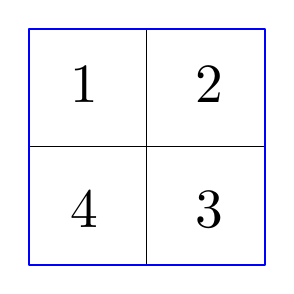
\begin{tikzpicture}[scale=.75, line join=round, line cap=round, >=stealth]
			\tikzset{every node/.style={thick,scale=2}}
			\def\R{2}  \def\r{.2} \def\d{1.5} 
			\path  (0,0)  coordinate (O) 
			(0:\R) coordinate (A)
			(90:\R) coordinate (B)
			(180:\R) coordinate (C)
			(-90:\R) coordinate (D)
			;
			\foreach \x in {A,B,C,D}{\draw (O)--(\x);}
			\draw[blue, thick] (-\R,-\R) rectangle (\R,\R);
			\draw (45:\d) node{$2$} (135:\d) node{$1$} (-135:\d) node{$4$} (-45:\d) node{$3$};
		\end{tikzpicture}
	\end{center}
	Có bao nhiêu cách để người thợ sơn có thể dùng bốn màu khác nhau để sơn tấm tường này sao cho mỗi ô vuông được tô một màu và những ô vuông cạnh nhau không có màu trùng nhau?
	\par
	\shortans{84}
	\loigiai{
		\begin{itemize}
			\item \textbf{Trường hợp $1$:} Ô số $1$ và ô số $3$ cùng màu.\\
			Chọn màu cho ô số $1$ có $4$ cách.\\ 
			Chọn màu cho ô số $3$ có $1$ cách.\\
			Hai ô số $2$ và $4$ đều có cùng số cách chọn là $3$.\\
			Số cách chọn màu trong trường hợp này là $4\cdot 1\cdot 3\cdot 3=36$.
			\item \textbf{Trường hợp $2$:} Ô số $1$ và ô số $3$ không cùng màu.\\
			Chọn màu cho ô số $1$ có $4$ cách. \\
			Chọn màu cho ô số $3$ có $3$ cách.\\
			Hai ô số $2$ và $4$ đều có cùng số cách chọn là $2$.\\
			Số cách chọn màu trong trường hợp này là $4\cdot 3\cdot 2\cdot 2=48$.
		\end{itemize}
		Vậy số cách chọn màu thỏa mãn là $36+48=84$.
	}
\end{ex}
%-----Câu 5
\begin{ex}%[0D8V1-5]%[Biên soạn tài liệu dạy học bộ KNTT-CS]%[GV Lien Nguyen]
	Từ các chữ số $0$, $1$, $2$, $3$, $4$, $5$ có thể lập được bao nhiêu số tự nhiên gồm bốn chữ số phân biệt và chia hết cho $4$?
	\par
	\shortans{72}
	\loigiai{
		Gọi số tự nhiên cần tìm là $\overline{abcd}$.\\
		\textbf{Nhận xét:} Một số tự nhiên (gồm nhiều chữ số) chia hết cho $4$ khi hai chữ số cuối của nó hình thành một số tư nhiên chia hết cho $4$.\\
		Theo đề, ta có $\overline{cd} \in  \{04,12,20,24,32,40,52\}$.\\
		\textbf{Trường hợp $1$:} $\overline{c d} \in\{04,20,40\}$, có $3$ cách chọn $\overline{c d}$.\\
		Chọn $a$ có $4$ cách; chọn $b$ có $3$ cách.\\
		Vậy số các số thỏa mãn là $3 \cdot 4 \cdot 3=36$ (số).\\
		\textbf{Trường hợp $2$:} $\overline{cd} \in\{12,24,32,52\}$, có $4$ cách chọn.\\
		Chọn $a$ có $3$ cách; chọn $b$ có $3$ cách. Số các số thỏa mãn là $4\cdot 3 \cdot 3=36$.\\
		Vậy số các số tự nhiên thỏa đề bài là $36+36=72$ (số).
	}
\end{ex}
%-----Câu 6
\begin{ex}%[0D8V1-2]%[Biên soạn tài liệu dạy học bộ KNTT-CS]%[GV Lien Nguyen]
	Cho $11$ điểm phân biệt. Hỏi có bao nhiêu đường thẳng được tạo ra từ $11$ điểm này?
		\par
	\shortans{55}
	\loigiai{
		Một đường thẳng được xác định nếu biết hai điểm thuộc đường thẳng.\\
		Có $11$ cách chọn điểm thứ nhất và $10$ cách chọn điểm thứ hai.\\
		Vì đường thẳng $AB$ và $BA$ là hai đường thẳng trùng nhau nên mỗi số đường thẳng được tạo ra là $\dfrac{11\cdot 10}{2}=55$ đường thẳng.
	}
\end{ex}

\Closesolutionfile{ans}
%------------------Tự luận
\ind{PHẦN IV.} \inden{Tự luận.}
\setcounter{ex}{0}
%-----Bài 1
\begin{ex}%[0D8H1-5]%[Biên soạn tài liệu dạy học bộ KNTT-CS]%[GV Lien Nguyen]
	Có bao nhiêu số tự nhiên có ba chữ số, trong đó chữ số hàng trăm là chữ số chẵn, chữ số hàng đơn vị là chữ số lẻ?
	\loigiai{
		Ký hiệu số cần lập là $\overline{abc}$.\\
		Chữ số hàng trăm là số chẵn nên $a$ có $4$ cách chọn ($2$, $4$, $6$ hoặc $8$).\\
		Chữ số hàng đơn vị là số lẻ nên $c$ có $5$ cách chọn ($1$, $3$, $5$, $7$ hoặc $9$).\\
		Vị trí $b$ có $10$ cách chọn.\\
		Áp dụng quy tắc nhân, có $4 \cdot 5 \cdot 10 = 200$ số thỏa yêu cầu đề bài.
	}
\end{ex}
%-----Bài 2
\begin{ex}%[0D8H1-3]%[Biên soạn tài liệu dạy học bộ KNTT-CS]%[GV Lien Nguyen]
	An có thể đi từ nhà đến trường theo các con đường như hình dưới, trong đó có những con đường đi qua nhà sách.
	\begin{center}
		\begin{tikzpicture}[scale=1, font=\footnotesize, line join=round, line cap=round, >=stealth]
			\tkzDefPoints{0/0/A,3/0/B,6/0/C}
			\draw (C) arc [start angle=0, end angle=180, x radius=3, y radius=1];
			\draw (C) arc [start angle=0, end angle=-180, x radius=3, y radius=1];
			\draw (B) arc [start angle=0, end angle=180, x radius=3/2, y radius=1/2];
			\draw (B) arc [start angle=0, end angle=-180, x radius=3/2, y radius=1/2];
			\draw (C) arc [start angle=0, end angle=180, x radius=3/2, y radius=1/2];
			\draw (C) arc [start angle=0, end angle=-180, x radius=3/2, y radius=1/2];
			\draw (A) -- (B);
			\filldraw (A) circle (0.05) (B) circle (0.05) (C) circle (0.05);
			\draw (A) node[left]{Nhà An} (B) node[below=0.4]{Nhà sách} (C) node[right]{Trường};
		\end{tikzpicture}
	\end{center}
	\begin{enumerate}
		\item An có bao nhiêu cách đi từ nhà đến trường mà có đi qua nhà sách?
		\item An có bao nhiêu cách đi từ nhà đến trường?
	\end{enumerate}
	Lưu ý: Chỉ tính những con đường đi qua các điểm (nhà An, nhà sách, trường) không quá một lần.
	\loigiai{
		\begin{enumerate}
			\item Công việc gồm hai bước:\\
			\textit{Bước $1$:} Đi từ nhà An đến nhà sách, có $3$ con đường.\\
			\textit{Bước $2$:} Đi từ nhà sách đến trường, có $2$ con đường.\\
			Áp dụng quy tắc nhân, có $3 \cdot 2 = 6$ con đường để An đi từ nhà đến trường mà có đi qua nhà sách.
			\item Công việc có hai phương án thực hiện:\\
			\textit{Phương án $1$:} An đi qua nhà sách, theo câu a, có $6$ con đường.\\
			\textit{Phương án $2$:} An không đi qua nhà sách, có $2$ con đường.\\
			Áp dụng quy tắc cộng, An có $6 + 2 = 8$ con đường đi từ nhà đến trường.
		\end{enumerate}
	}
\end{ex}	
%-----Bài 3
\begin{ex}%[0D8H1-2]%[Biên soạn tài liệu dạy học bộ KNTT-CS]%[GV Lien Nguyen]
	Một thùng chứa $6$ quả dưa hấu, một thùng khác chứa $15$ quả thanh long. Từ hai thùng này,
	\begin{enumerate}
		\item có bao nhiêu cách chọn một quả dưa hấu hoặc một quả thanh long?
		\item có bao nhiêu cách chọn một quả dưa hấu và một quả thanh long?
	\end{enumerate}	
	\loigiai{
		\begin{enumerate}
			\item Công việc có hai phương án thực hiện:\\
			\textit{Phương án $1$:} Chọn một quả dưa hấu, có $6$ cách chọn.\\
			\textit{Phương án $2$:} Chọn một quả thanh long, có $15$ cách chọn.\\
			Áp dụng quy tắc cộng, có $6+15=21$ cách thực hiện.
			\item Công việc có hai công đoạn thực hiện:\\
			\textit{Công đoạn thứ nhất:} Chọn một quả dưa hấu, có $6$ cách chọn.\\
			\textit{Công đoạn thứ hai:} Chọn một quả thanh long, có $15$ cách chọn.\\
			Áp dụng quy tắc nhân, có $6 \cdot 15= 90$ cách thực hiện.
		\end{enumerate}
	}
\end{ex}
%-----Bài 4
\begin{ex}%[0D8V1-1]%[Biên soạn tài liệu dạy học bộ KNTT-CS]%[GV Lien Nguyen]
	Tính số giao điểm tối đa của $10$ đường thẳng phân biệt khi không có ba đường nào đồng quy và hai đường nào song song?
	\loigiai{
		Đường thẳng thứ nhất giao với $9$ đường còn lại nên có $9$ giao điểm.\\
		Đường thẳng thứ hai giao với $8$ đường còn lại nên có thêm $8$ giao điểm (đã tính giao điểm với đường thẳng thứ nhất ở trên).\\
		Đường thẳng thứ $9$ giao với $1$ đường còn lại nên có thêm $1$ giao điểm.\\ 
		Vậy có $9+8+7+6+5+4+3+2+1=45$ giao điểm.
	}
\end{ex}
%-----Bài 5
\begin{ex}%[0D8H1-1][Biên soạn tài liệu dạy học bộ KNTT-CS]%[GV Lien Nguyen]
	Giả sử từ tỉnh $A$ đến tỉnh $B$ có thể đi bằng các phương tiện: ô tô, tàu hỏa, tàu thủy hoặc máy bay. Mỗi ngày có $8$ chuyến ô tô, $4$ chuyến tàu hỏa, $2$ chuyến tàu thủy và $2$ chuyến máy bay. Hỏi có bao nhiêu cách đi từ tỉnh $A$ đến tỉnh $B$ bằng một trong các phương tiện trên?
	\loigiai{
		Việc di chuyển từ tỉnh $A$ đến tỉnh $B$ có bốn phương án thực hiện:\\
		Di chuyển bằng ô tô, có $8$ cách chọn chuyến.\\
		Di chuyển bằng tàu hỏa, có $4$ cách chọn chuyến.\\
		Di chuyển bằng tàu thủy, có $2$ cách chọn chuyến.\\
		Di chuyển bằng máy bay, có $2$ cách chọn chuyến.\\
		Áp dụng quy tắc cộng, ta có số cách chọn để di chuyển từ $A$ đến $B$ là $8+4+2+2=16$ cách.
	}
\end{ex}
%-----Bài 6
\begin{ex}%[0D8V1-2]%[Biên soạn tài liệu dạy học bộ KNTT-CS]%[GV Lien Nguyen]
	Biển số xe máy của tỉnh $A$ (nếu không kể mã số tỉnh) có $6$ kí tự, trong đó kí tự ở vị trí đầu tiên là một chữ cái (trong bảng $26$ cái tiếng Anh), kí tự ở vị trí thứ hai là một chữ số thuộc tập $\{1; 2; \ldots; 9\}$ mỗi kí tự ở bốn vị trí tiếp theo là một chữ số thuộc tập $\{0; 1; 2; \ldots; 9\}$. Hỏi nếu chỉ dùng một mã số tỉnh thì tỉnh $A$ có thể làm được nhiều nhất bao nhiêu biển số xe máy khác nhau?
	\loigiai{
		Giả sử biển số xe là $\overline{abcdef}$.\\ 
		Có $26$ cách chọn $a$;\\ 
		Có $9$ cách chọn $b$;\\ 
		Có $10$ cách chọn $c$;\\ 
		Có $10$ cách chọn $d$;\\ 
		Có $10$ cách chọn $e$;\\ 
		Có $10$ cách chọn $f$.\\ 
		Vậy có $26\cdot 9\cdot 10\cdot 10\cdot 10\cdot 10=2\,340\,000$ biển số xe.
	}
\end{ex}
\Closesolutionfile{ans}


\subsection{HOÁN VỊ - CHỈNH HỢP - TỔ HỢP}
%-------------Trắc nghiệm nhiều lựa chọn
\ind{PHẦN I.} \inden{Câu trắc nghiệm nhiều phương án lựa chọn. Mỗi câu hỏi học sinh chỉ chọn một phương án.}
\setcounter{ex}{0}
\Opensolutionfile{ans}[ans/ans-c8b24-lc]
\begin{ex}%[0D8N2-7]%[Biên soạn tài liệu dạy học bộ KNTT-CS]%[GV biên soạn: Mai Thái Phong]
	Có bao nhiêu cách sắp xếp $5$ học sinh thành một hàng dọc?
	\choice
	{$5$}
	{$10$}
	{\True $\mathrm{P}_5$}
	{$5^5$}
	\loigiai
	{
		Mỗi cách sắp xếp $5$ học sinh thành một hàng dọc là một hoán vị của $5$ phần tử.\\
		Số cách sắp xếp là $\mathrm{P}_5 = 5! = 120$ cách.
	}
\end{ex}
\begin{ex}%[0D8N2-2]%[Biên soạn tài liệu dạy học bộ KNTT-CS]%[GV biên soạn: Mai Thái Phong]
	Cho tập hợp $A$ có $n$ phần tử ($n \in \mathbb{N}, n \ge 1$). Số hoán vị của $n$ phần tử là
	\choice
	{\True $n!$}
	{$n^n$}
	{$2^n$}
	{$n^2$}
	\loigiai
	{
		Theo định nghĩa, số các hoán vị của tập hợp có $n$ phần tử là $\mathrm{P}_n = n!$.
	}
\end{ex}
\begin{ex}%[0D8N2-2]%[Biên soạn tài liệu dạy học bộ KNTT-CS]%[GV biên soạn: Mai Thái Phong]
	Số các chỉnh hợp chập $k$ của $n$ phần tử ($1 \le k \le n$) được tính bởi công thức nào sau đây?
	\choice
	{$\mathrm{A}_n^k = \dfrac{n!}{k!}$}
	{\True $\mathrm{A}_n^k = \dfrac{n!}{(n-k)!}$}
	{$\mathrm{A}_n^k = \dfrac{n!}{k!(n-k)!}$}
	{$\mathrm{A}_n^k = \dfrac{(n-k)!}{n!}$}
	\loigiai
	{
		Số các chỉnh hợp chập $k$ của $n$ phần tử là $\mathrm{A}_n^k = \dfrac{n!}{(n-k)!}$.
	}
\end{ex}
\begin{ex}%[0D8N2-3]%[Biên soạn tài liệu dạy học bộ KNTT-CS]%[GV biên soạn]
	Từ các chữ số $\{1, 2, 3, 4, 5\}$, có thể lập được bao nhiêu số tự nhiên có $3$ chữ số khác nhau?
	\choice
	{$\mathrm{C}_5^3$}
	{$5^3$}
	{\True $\mathrm{A}_5^3$}
	{$3^5$}
	\loigiai
	{
		Mỗi số tự nhiên có $3$ chữ số khác nhau được lập từ $5$ chữ số đã cho là một chỉnh hợp chập $3$ của $5$ phần tử.\\
		Số các số lập được là $\mathrm{A}_5^3 = 60$ số.
	}
\end{ex}
\begin{ex}%[0D8N2-2]]%[Biên soạn tài liệu dạy học bộ KNTT-CS]%[GV biên soạn: Mai Thái Phong]
	Số các tổ hợp chập $k$ của $n$ phần tử ($0 \le k \le n$) là
	\choice
	{$\mathrm{C}_n^k = \dfrac{n!}{(n-k)!}$}
	{$\mathrm{C}_n^k = \dfrac{n!}{k!}$}
	{\True $\mathrm{C}_n^k = \dfrac{n!}{k!(n-k)!}$}
	{$\mathrm{C}_n^k = \dfrac{(n-k)!}{k!n!}$}
	\loigiai
	{
		Công thức tính số tổ hợp chập $k$ của $n$ phần tử là $\mathrm{C}_n^k = \dfrac{n!}{k!(n-k)!}$.
	}
\end{ex}
\begin{ex}%[0D8N2-4]%[Biên soạn tài liệu dạy học bộ KNTT-CS]%[GV biên soạn: Mai Thái Phong]
	Một tổ có $10$ học sinh. Số cách chọn ra $2$ học sinh đi trực nhật là
	\choice
	{$\mathrm{A}_{10}^2$}
	{\True $\mathrm{C}_{10}^2$}
	{$10^2$}
	{$20$}
	\loigiai
	{
		Vì việc chọn $2$ học sinh không phân biệt thứ tự nên mỗi cách chọn là một tổ hợp chập $2$ của $10$ phần tử.\\
		Số cách chọn là $\mathrm{C}_{10}^2 = 45$ cách.
	}
\end{ex}
\begin{ex}%[0D8H2-7]%[Biên soạn tài liệu dạy học bộ KNTT-CS]%[GV biên soạn: Mai Thái Phong]
	Có bao nhiêu số tự nhiên gồm $4$ chữ số khác nhau được lập từ các chữ số $1$, $2$, $3$, $4$, $5$, $6$?
	\choice
	{$4^6$}
	{$6^4$}
	{$15$}
	{\True $360$}
	\loigiai
	{
		Mỗi số tự nhiên gồm $4$ chữ số khác nhau lập từ tập hợp $6$ chữ số đã cho là một chỉnh hợp chập $4$ của $6$ phần tử.\\
		Số các số cần tìm là $\mathrm{A}_6^4 = \dfrac{6!}{(6-4)!} = 360$ số.
	}
\end{ex}
\begin{ex}%[0D8H2-6]%[Biên soạn tài liệu dạy học bộ KNTT-CS]%[GV biên soạn: Mai Thái Phong]
	Trong một mặt phẳng cho $10$ điểm phân biệt, trong đó không có $3$ điểm nào thẳng hàng. Có thể lập được bao nhiêu tam giác có các đỉnh là $3$ trong $10$ điểm đã cho?
	\choice
	{\True $120$}
	{$720$}
	{$30$}
	{$10^3$}
	\loigiai
	{
		Mỗi tam giác được hình thành bằng cách chọn $3$ điểm không thẳng hàng từ $10$ điểm đã cho. Vì không có $3$ điểm nào thẳng hàng nên số tam giác là $\mathrm{C}_{10}^3$.\\
		Ta có $\mathrm{C}_{10}^3 = \dfrac{10 \cdot 9 \cdot 8}{3 \cdot 2 \cdot 1} = 120$ tam giác.
	}
\end{ex}
\begin{ex}%[0D8H2-4]%[Biên soạn tài liệu dạy học bộ KNTT-CS]%[GV biên soạn: Mai Thái Phong]
	Một nhóm công nhân gồm $7$ nam và $3$ nữ. Có bao nhiêu cách chọn một đội công tác gồm $5$ người sao cho có đúng $2$ nữ?
	\choice
	{\True $105$}
	{$21$}
	{$35$}
	{$120$}
	\loigiai
	{
		Để chọn đội công tác có đúng $2$ nữ, ta thực hiện hai công đoạn:
		\begin{itemize}
			\item Chọn $2$ nữ từ $3$ nữ có $\mathrm{C}_3^2 = 3$ cách.
			\item Chọn $3$ nam từ $7$ nam (để đủ $5$ người) có $\mathrm{C}_7^3 = 35$ cách.
		\end{itemize}
		Theo quy tắc nhân, số cách chọn là $3 \cdot  35 = 105$ cách.
	}
\end{ex}
\begin{ex}%[0D8H2-2]%[Biên soạn tài liệu dạy học bộ KNTT-CS]%[GV biên soạn: Mai Thái Phong]
	Một hộp chứa $10$ quả cầu gồm $6$ quả cầu màu đỏ và $4$ quả cầu màu xanh. Có bao nhiêu cách chọn ra $3$ quả cầu từ hộp đó sao cho có đúng $2$ quả cầu màu đỏ?
	\choice
	{$\mathrm{C}_{10}^3$}
	{$24$}
	{\True $60$}
	{$120$}
	\loigiai
	{
		Để chọn được $3$ quả cầu trong đó có đúng $2$ quả cầu màu đỏ, ta thực hiện qua hai công đoạn liên tiếp sau:
		\begin{itemize}
			\item Công đoạn 1: Chọn $2$ quả cầu màu đỏ từ $6$ quả cầu màu đỏ. Số cách chọn là $\mathrm{C}_6^2 = 15$ cách.
			\item Công đoạn 2: Chọn $1$ quả cầu màu xanh từ $4$ quả cầu màu xanh (để đủ số lượng $3$ quả cầu). Số cách chọn là $\mathrm{C}_4^1 = 4$ cách.
		\end{itemize}
		Theo quy tắc nhân, số cách chọn thỏa mãn yêu cầu bài toán là $15 \cdot  4 = 60$ cách.
	}
\end{ex}
\begin{ex}%[0D8H2-7]%[Biên soạn tài liệu dạy học bộ KNTT-CS]%[GV biên soạn: Mai Thái Phong]
	Có bao nhiêu cách sắp xếp $3$ học sinh nam và $3$ học sinh nữ vào một dãy ghế hàng ngang có $6$ chỗ ngồi sao cho các học sinh nam và nữ ngồi xen kẽ nhau?
	\choice
	{$36$}
	{$144$}
	{\True $72$}
	{$48$}
	\loigiai
	{
		Có $2$ trường hợp ngồi xen kẽ:\\
		Trường hợp 1: Nam ngồi các vị trí lẻ ($1, 3, 5$), nữ ngồi các vị trí chẵn ($2, 4, 6$).
		\begin{itemize}
			\item Xếp nam có $3!$ cách.
			\item Xếp nữ có $3!$ cách.
			\item Số cách là $3! \cdot  3! = 36$ cách.
		\end{itemize}
		Trường hợp 2: Nữ ngồi các vị trí lẻ, nam ngồi các vị trí chẵn. Tương tự có $3! \cdot  3! = 36$ cách.\\
		Tổng cộng có $36 + 36 = 72$ cách.
	}
\end{ex}
\begin{ex}%[0D8H2-5]%[Biên soạn tài liệu dạy học bộ KNTT-CS]%[GV biên soạn: Mai Thái Phong]
	Một hộp chứa $6$ viên bi đỏ và $4$ viên bi xanh. Có bao nhiêu cách chọn ra $4$ viên bi sao cho có ít nhất một viên bi xanh?
	\choice
	{$195$}
	{\True $195$}
	{$210$}
	{$209$}
	\loigiai
	{
		Tổng số cách chọn $4$ viên bi bất kì từ $10$ viên bi là $\mathrm{C}_{10}^4 = 210$ cách.\\
		Số cách chọn $4$ viên bi mà không có viên bi xanh nào (tức là cả $4$ viên đều đỏ) là $\mathrm{C}_6^4 = 15$ cách.\\
		Số cách chọn có ít nhất một viên bi xanh là $210 - 15 = 195$ cách.
	}
\end{ex}
\Closesolutionfile{ans}
\indapan{6}{ans/ans-c8b24-lc}
%---------------------Trắc nghiệm đúng sai
\ind{PHẦN II.} \inden{Câu trắc nghiệm đúng sai. Trong mỗi ý a), b), c), d) ở mỗi câu, học sinh chọn đúng hoặc sai.}
\setcounter{ex}{0}
\Opensolutionfile{ans}[ans/ans-c8b24-ds]
\begin{ex}%[0D8N2-3]%[Biên soạn tài liệu dạy học bộ KNTT-CS]%[GV biên soạn: Mai Thái Phong]
	Cho tập hợp $A = \{1, 2, 3, 4, 5, 6\}$. Xét các khẳng định sau
	\choiceTF
	{Số các số tự nhiên có $6$ chữ số đôi một khác nhau lập từ tập $A$ là $\mathrm{P}_6 = 720$}
	{\True Số tập con có $3$ phần tử của tập $A$ là $\mathrm{C}_6^3 = 20$}
	{Số các số tự nhiên có $3$ chữ số đôi một khác nhau lập từ tập $A$ là $\mathrm{C}_6^3$}
	{\True Số cách chọn ra $2$ chữ số từ tập $A$ và sắp xếp chúng theo một thứ tự là $\mathrm{A}_6^2 = 30$}
	\loigiai
	{
		\begin{itemchoice}
			\itemch Mỗi số tự nhiên có $6$ chữ số đôi một khác nhau lập từ $6$ phần tử của $A$ là một hoán vị của $6$ phần tử. Số các số đó là $\mathrm{P}_6 = 6! = 720$.
			\itemch Mỗi tập con có $3$ phần tử của $A$ là một tổ hợp chập $3$ của $6$ phần tử. Số tập con là $\mathrm{C}_6^3 = \dfrac{6!}{3! \cdot 3!} = 20$.
			\itemch Số các số tự nhiên có $3$ chữ số đôi một khác nhau lập từ $A$ phải là một chỉnh hợp chập $3$ của $6$, tức là $\mathrm{A}_6^3 = 120$.
			\itemch Việc chọn $2$ chữ số và sắp xếp thứ tự là một chỉnh hợp chập $2$ của $6$ phần tử, số cách là $\mathrm{A}_6^2 = \dfrac{6!}{4!} = 30$.
		\end{itemchoice}
	}
\end{ex}
\begin{ex}%[0D8H2-4]%[Biên soạn tài liệu dạy học bộ KNTT-CS]%[GV biên soạn: Mai Thái Phong]
	Trong một giải thi đấu cầu lông có $10$ vận động viên tham gia thi đấu vòng tròn một lượt (hai vận động viên bất kỳ đều gặp nhau đúng một trận).
	\choiceTF
	{\True Tổng số trận đấu của giải là $\mathrm{C}_{10}^2$}
	{Số cách chọn ra $3$ vận động viên để trao giải Nhất, Nhì, Ba là $\mathrm{C}_{10}^3$}
	{\True Nếu có $2$ vận động viên bỏ cuộc trước khi giải bắt đầu thì số trận đấu giảm đi $17$ trận}
	{Số cách phân công $10$ vận động viên vào $5$ sân thi đấu khác nhau, mỗi sân $2$ người là $10!$}
	\loigiai
	{
		\begin{itemchoice}
			\itemch Mỗi trận đấu là một cách chọn $2$ vận động viên từ $10$ vận động viên (không tính thứ tự), nên số trận đấu là $\mathrm{C}_{10}^2 = 45$.
			\itemch Vì các giải Nhất, Nhì, Ba có phân biệt thứ tự nên số cách chọn là một chỉnh hợp chập $3$ của $10$, tức là $\mathrm{A}_{10}^3 = 720$.
			\itemch Nếu còn $8$ vận động viên, số trận đấu là $\mathrm{C}_8^2 = 28$. Số trận giảm đi là $45 - 28 = 17$.
			\itemch Việc phân công này phức tạp hơn và không đơn thuần là $10!$ (hoán vị $10$ phần tử).
		\end{itemchoice}
	}
\end{ex}
\begin{ex}%[0D8H2-4]%[Biên soạn tài liệu dạy học bộ KNTT-CS]%[GV biên soạn: Mai Thái Phong]
	Một đội văn nghệ có $7$ học sinh nam và $5$ học sinh nữ. Nhà trường cần chọn ra $5$ học sinh để đi biểu diễn.
	\choiceTF
	{Số cách chọn $5$ học sinh bất kỳ là $\mathrm{A}_{12}^5$}
	{\True Số cách chọn $5$ học sinh sao cho có đúng $3$ nam và $2$ nữ là $\mathrm{C}_7^3 \cdot \mathrm{C}_5^2$}
	{Số cách chọn $5$ học sinh sao cho có ít nhất $1$ học sinh nữ là $\mathrm{C}_{12}^5 - \mathrm{C}_5^5$}
	{\True Số cách chọn $5$ học sinh sao cho có ít nhất $1$ học sinh nữ là $771$ cách}
	\loigiai
	{
		\begin{itemchoice}
			\itemch Chọn $5$ học sinh từ $12$ học sinh không phân biệt thứ tự phải dùng tổ hợp $\mathrm{C}_{12}^5 = 792$.
			\itemch Chọn $3$ nam từ $7$ nam có $\mathrm{C}_7^3$ cách, chọn $2$ nữ từ $5$ nữ có $\mathrm{C}_5^2$ cách. Theo quy tắc nhân ta có $\mathrm{C}_7^3 \cdot \mathrm{C}_5^2$ cách.
			\itemch Số cách chọn ít nhất $1$ nữ = (Tổng số cách chọn $5$ người) $-$ (Số cách chọn $5$ người toàn nam). Vậy phải là $\mathrm{C}_{12}^5 - \mathrm{C}_7^5$.
			\itemch Ta có $\mathrm{C}_{12}^5 - \mathrm{C}_7^5 = 792 - 21 = 771$.
		\end{itemchoice}
	}
\end{ex}
\begin{ex}%[0D8H2-5]%[Biên soạn tài liệu dạy học bộ KNTT-CS]%[GV biên soạn: Mai Thái Phong]
	Một hộp đựng $15$ viên bi đôi một khác nhau, trong đó có $6$ viên bi xanh, $5$ viên bi đỏ và $4$ viên bi vàng. Người ta chọn ngẫu nhiên đồng thời $4$ viên bi từ hộp đó. Xét các khẳng định sau:
	\choiceTF
	{Số cách chọn $4$ viên bi bất kỳ từ hộp là $\mathrm{A}_{15}^4$}
	{\True Số cách chọn $4$ viên bi sao cho chúng có cùng một màu là $21$ cách}
	{\True Số cách chọn $4$ viên bi sao cho có ít nhất một viên bi vàng là $\mathrm{C}_{15}^4 - \mathrm{C}_{11}^4$}
	{Số cách chọn $4$ viên bi sao cho có đúng $2$ viên bi đỏ là $\mathrm{C}_5^2 \cdot \mathrm{C}_{10}^2 = 540$ cách}
	\loigiai
	{
		\begin{itemchoice}
			\itemch Vì chọn đồng thời $4$ viên bi nên không tính thứ tự, số cách chọn phải là một tổ hợp chập $4$ của $15$, tức là $\mathrm{C}_{15}^4 = 1365$ cách.
			\itemch Để chọn $4$ viên bi cùng màu, ta có các trường hợp:
			\begin{itemize}
				\item Chọn $4$ viên xanh từ $6$ viên xanh: $\mathrm{C}_6^4 = 15$ cách.
				\item Chọn $4$ viên đỏ từ $5$ viên đỏ: $\mathrm{C}_5^4 = 5$ cách.
				\item Chọn $4$ viên vàng từ $4$ viên vàng: $\mathrm{C}_4^4 = 1$ cách.
			\end{itemize}
			Tổng số cách là $15 + 5 + 1 = 21$ cách.
			\itemch Ta dùng phương pháp biến cố đối. Tổng số cách chọn $4$ viên bất kỳ là $\mathrm{C}_{15}^4$. Số cách chọn $4$ viên mà không có viên bi vàng nào (tức là chọn từ $11$ viên xanh và đỏ) là $\mathrm{C}_{11}^4$. Vậy số cách chọn có ít nhất một viên bi vàng là $\mathrm{C}_{15}^4 - \mathrm{C}_{11}^4$.
			\itemch Chọn $2$ viên bi đỏ từ $5$ viên đỏ có $\mathrm{C}_5^2$ cách. Chọn $2$ viên bi còn lại từ $10$ viên bi (xanh và vàng) có $\mathrm{C}_{10}^2$ cách. Theo quy tắc nhân, số cách chọn là $\mathrm{C}_5^2 \cdot \mathrm{C}_{10}^2 = 10 \cdot 45 = 450$ cách.
		\end{itemchoice}
	}
\end{ex}
\Closesolutionfile{ans}
\indapan{3}{ans/ans-c8b24-ds}
%---------------Trắc nghiệm trả lời ngắn
\ind{PHẦN III.} \inden{Câu trả lời ngắn.}
\setcounter{ex}{0}
\Opensolutionfile{ans}[ans/ans-c1b1-kq]
%-----Câu 1
\begin{ex}%[0D8H2-7]%[Biên soạn tài liệu dạy học bộ KNTT-CS]%[GV biên soạn: Mai Thái Phong]
	Có bao nhiêu cách xếp $5$ học sinh thành một hàng dọc?
	\par
	\shortans{$120$}
	\loigiai
	{
		Mỗi cách xếp $5$ học sinh thành một hàng dọc là một hoán vị của $5$ phần tử.
		\\
		Số cách xếp là $\mathrm{P}_5 = 5! = 120$.
	}
\end{ex}
\begin{ex}%[0D8V2-4]%[Biên soạn tài liệu dạy học bộ KNTT-CS]%[GV biên soạn: Mai Thái Phong]
	Một nhóm tình nguyện gồm $10$ học sinh, trong đó có $6$ nam và $4$ nữ. Hỏi có bao nhiêu cách chọn ra $3$ học sinh sao cho trong đó có ít nhất một học sinh nữ?
	\par
	\shortans{$100$}
	\loigiai
	{
		Số cách chọn $3$ học sinh bất kì từ $10$ học sinh là $\mathrm{C}_{10}^3 = 120$. \\
		Số cách chọn $3$ học sinh mà không có học sinh nữ nào (tức là chọn $3$ nam từ $6$ nam) là $\mathrm{C}_6^3 = 20$. \\
		Số cách chọn có ít nhất một học sinh nữ là $120 - 20 = 100$.
	}
\end{ex}
\begin{ex}%[0D8H2-3]%[Biên soạn tài liệu dạy học bộ KNTT-CS]%[GV biên soạn: Mai Thái Phong]
	Một câu lạc bộ có $15$ thành viên. Có bao nhiêu cách chọn ra $2$ thành viên để bầu vào hai vị trí khác nhau là Chủ nhiệm và Phó chủ nhiệm?
	\shortans{210}
	\loigiai
	{
		Mỗi cách chọn ra $2$ thành viên từ $15$ thành viên và sắp xếp vào $2$ vị trí khác nhau (có phân biệt thứ tự) là một chỉnh hợp chập $2$ của $15$ phần tử. \\
		Số cách chọn là $\mathrm{A}_{15}^2 = 15 \cdot  14 = 210$.
	}
\end{ex}
\begin{ex}%[0D8V2-5]%[Biên soạn tài liệu dạy học bộ KNTT-CS]%[GV biên soạn: Mai Thái Phong]
	Trên một kệ sách có $4$ cuốn sách Toán khác nhau và $3$ cuốn sách Vật lý khác nhau. Hỏi có bao nhiêu cách sắp xếp các cuốn sách thành một hàng ngang sao cho các cuốn sách cùng môn luôn đứng cạnh nhau?
	\par
	\shortans{$288$}
	\loigiai
	{
		Xem nhóm sách Toán là một vật thể $X$, nhóm sách Vật lý là một vật thể $Y$. \\
		Số cách xếp $X$ và $Y$ là $2! = 2$ cách. \\
		Trong nhóm $X$, số cách xếp $4$ cuốn Toán là $4! = 24$ cách. \\
		Trong nhóm $Y$, số cách xếp $3$ cuốn Vật lý là $3! = 6$ cách. \\
		Vậy tổng số cách xếp là $2 \cdot  24 \cdot  6 = 288$.
	}
\end{ex}
\begin{ex}%[0D8V2-4]%[Biên soạn tài liệu dạy học bộ KNTT-CS]%[GV biên soạn: Mai Thái Phong]
	Trong một buổi gặp mặt giữa các đại biểu, mỗi người đều bắt tay với tất cả những người còn lại một lần. Biết rằng có tất cả $190$ cái bắt tay, hỏi buổi gặp mặt đó có bao nhiêu đại biểu tham dự?
	\par
	\shortans{$20$}
	\loigiai
	{
		Gọi $n$ là số đại biểu tham dự ($n \in \mathbb{N}, n \ge 2$). \\
		Mỗi cái bắt tay là một cách chọn ra $2$ người từ $n$ người, tức là một tổ hợp chập $2$ của $n$ phần tử. \\
		Theo đề bài ta có phương trình $\mathrm{C}_n^2 = 190 \Leftrightarrow \dfrac{n(n-1)}{2} = 190 \Leftrightarrow n^2 - n - 380 = 0$. \\
		Giải phương trình ta được $n = 20$ (thỏa mãn) hoặc $n = -19$ (loại). \\
		Vậy có $20$ đại biểu.
	}
\end{ex}
\begin{ex}%[0D8C2-3]%[Biên soạn tài liệu dạy học bộ KNTT-CS]%[GV biên soạn: Mai Thái Phong]
	Có bao nhiêu số tự nhiên có $5$ chữ số đôi một khác nhau được lập từ tập hợp \break $A = \{0,\,1,\,2,\,3,\,4,\,5\}$ sao cho các chữ số lẻ luôn đứng cạnh nhau?
	\par
	\shortans{$84$}
	\loigiai
	{
		Tập $A$ có các chữ số lẻ là $L = \{1, 3, 5\}$ và các chữ số chẵn là $C = \{0, 2, 4\}$. \\
		Vì số có $5$ chữ số khác nhau nên ta chọn thêm $2$ chữ số từ tập $C$. \\
		Nhóm $3$ chữ số lẻ thành một khối $X$, có $3! = 6$ cách xếp các chữ số lẻ trong $X$. \\
		Trường hợp 1: Chọn thêm $2$ chữ số từ $\{2, 4\}$. Khi đó có $1$ cách chọn. Hoán vị $X$ và $\{2, 4\}$ có $3!$ cách. Số các số là $1 \cdot  6 \cdot  3! = 36$. \\
		Trường hợp 2: Chọn thêm chữ số $0$ và một chữ số từ $\{2, 4\}$. Có $\mathrm{C}_2^1 = 2$ cách chọn. Hoán vị $X, 0$ và chữ số còn lại có $3!$ cách, trong đó có $2!$ cách mà số $0$ đứng đầu. \\
		Số các số là $2 \cdot  6 \cdot  (3! - 2!) = 12 \cdot  4 = 48$. \\
		Tổng cộng có $36 + 48 = 84$ số.
	}
\end{ex}
\Closesolutionfile{ans}
\indapan{4}{ans/ans-c1b1-kq}
%------------------Tự luận
\ind{PHẦN IV.} \inden{Tự luận.}
\setcounter{ex}{0}
\begin{ex}%[0D8V2-4]%[Biên soạn tài liệu dạy học bộ KNTT-CS]%[GV biên soạn: Mai Thái Phong]
	Một đội văn nghệ có $10$ học sinh nam và $6$ học sinh nữ. Chọn ngẫu nhiên $5$ học sinh để đi biểu diễn. Hỏi có bao nhiêu cách chọn sao cho trong $5$ học sinh được chọn có ít nhất $2$ học sinh nữ?
	\loigiai
	{
		Tổng số cách chọn $5$ học sinh từ $16$ học sinh là $\mathrm{C}_{16}^5 = 4\,368$ cách. \\
		Ta sử dụng phương pháp phần bù
		\begin{itemize}
			\item Trường hợp không có học sinh nữ nào (chọn $5$ nam) có $\mathrm{C}_{10}^5 = 252$ cách.
			\item Trường hợp có đúng $1$ học sinh nữ (chọn $1$ nữ và $4$ nam) có $\mathrm{C}_6^1 \cdot \mathrm{C}_{10}^4 = 6 \cdot 210 = 1\,260$ cách.
		\end{itemize}
		Số cách chọn có ít nhất $2$ học sinh nữ là
		$$ 4\,368 - (252 + 1\,260) = 2\,856 \text{ cách.} $$
	}
\end{ex}
\begin{ex}%[0D8H2-5]%[Biên soạn tài liệu dạy học bộ KNTT-CS]%[GV biên soạn: Mai Thái Phong]
Bạn Nam có $4$ quyển sách Toán, $6$ quyển sách Tiếng Anh (các quyển sách là khác nhau). Hỏi có bao nhiêu cách xếp các quyển sách thành hàng ngang sao cho:
\begin{enumerate}
	\item Các quyển sách cùng môn thì xếp cạnh nhau (không có quyển sách Toán nào nằm giữa hai quyển sách Tiếng Anh và ngược lại)?
	\item Các quyển sách Toán thì xếp cạnh nhau?
\end{enumerate}
\loigiai{
	\begin{enumerate}
		\item Xếp $4$ quyển sách Toán cạnh nhau thành một nhóm có $\mathrm{P}_4 = 4! = 24$ (cách).\\
		Xếp $6$ quyển sách Tiếng Anh cạnh nhau thành một nhóm có $\mathrm{P}_6 = 6! = 720$ (cách).\\
		Có $\mathrm{P}_2 = 2! = 2$ cách xếp hai nhóm trên.\\
		Vậy số cách xếp các quyển sách sao cho các quyển sách cùng môn thì xếp cạnh nhau là
		$24 \cdot 720 \cdot 2 = 34\,560$.
		\item Xếp $4$ quyển sách Toán cạnh nhau thành một nhóm có $\mathrm{P}_4 = 4! = 24$ (cách).\\
		Coi nhóm sách Toán là một quyển sách, gọi là $A$, xếp quyển sách A và $6$ quyển sách Tiếng Anh có $\mathrm{P}_7 = 7! = 5\,040$ (cách).\\
		Vậy số cách xếp các quyển sách sao cho các quyển sách Toán thì xếp cạnh nhau là $24 \cdot 5\,040 = 120\,960$.
	\end{enumerate}	
}
\end{ex}
\begin{ex}%[0D8C2-3]%[Biên soạn tài liệu dạy học bộ KNTT-CS]%[GV biên soạn: Mai Thái Phong]
	Có bao nhiêu số tự nhiên có $7$ chữ số được lập từ các chữ số $\{1,\,2,\,3,\,4,\,5\}$ sao cho chữ số $1$ xuất hiện đúng $3$ lần, các chữ số còn lại xuất hiện đúng $1$ lần?
	\loigiai
	{
		Số các số thỏa mãn yêu cầu là số cách sắp xếp $7$ chữ số, trong đó có $3$ chữ số $1$ và $4$ chữ số khác nhau là $\{2,\,3,\,4,\,5\}$.
		\begin{itemize}
			\item Bước 1: Chọn $3$ vị trí trong $7$ vị trí để đặt chữ số $1$, có $\mathrm{C}_7^3 = 35$ cách.
			\item Bước 2: Còn lại $4$ vị trí trống, ta xếp $4$ chữ số $\{2,\,3,\,4,\,5\}$ vào đó. Đây là một hoán vị của $4$ phần tử, có $\mathrm{P}_4 = 4! = 24$ cách.
		\end{itemize}
		Vậy số các số tự nhiên thỏa mãn là $35 \cdot  24 = 840$ số.
	}
\end{ex}
\begin{ex}%[0D8H2-6]%[Biên soạn tài liệu dạy học bộ KNTT-CS]%[GV biên soạn: Mai Thái Phong]
	Trong mặt phẳng cho hai đường thẳng song song $d_1$ và $d_2$. Trên đường thẳng $d_1$ lấy $10$ điểm phân biệt, trên đường thẳng $d_2$ lấy $8$ điểm phân biệt.
	\begin{enumerate}
		\item Có bao nhiêu đoạn thẳng có hai đầu mút được chọn từ $18$ điểm đã cho?
		\item Có bao nhiêu tam giác có các đỉnh được chọn từ $18$ điểm đã cho?
		\item Có bao nhiêu hình thang có các đỉnh được chọn từ $18$ điểm đã cho?
	\end{enumerate}
	\loigiai
	{
		\begin{enumerate}
			\item Một đoạn thẳng được xác định bằng cách chọn $2$ điểm bất kì từ $18$ điểm đã cho ($10 + 8 = 18$). \\
			Số đoạn thẳng là $\mathrm{C}_{18}^2 = 153$ (đoạn thẳng).		
			\item Để tạo thành một tam giác, ta không thể chọn $3$ điểm thẳng hàng. Có $2$ trường hợp:
			\begin{itemize}
				\item Trường hợp 1: Chọn $2$ điểm từ $d_1$ và $1$ điểm từ $d_2$. \\
				Số cách chọn: $\mathrm{C}_{10}^2 \cdot \mathrm{C}_8^1 = 45 \cdot 8 = 360$ (tam giác).
				\item Trường hợp 2: Chọn $1$ điểm từ $d_1$ và $2$ điểm từ $d_2$. \\
				Số cách chọn: $\mathrm{C}_{10}^1 \cdot \mathrm{C}_8^2 = 10 \cdot 28 = 280$ (tam giác).
			\end{itemize}
			Tổng số tam giác tạo thành là $360 + 280 = 640$ (tam giác).
			
			\item Một hình thang có hai đáy nằm trên $d_1$ và $d_2$. Để tạo thành hình thang, ta cần chọn $2$ điểm từ $d_1$ (làm đáy thứ nhất) và $2$ điểm từ $d_2$ (làm đáy thứ hai). \\
			Số hình thang tạo thành là $\mathrm{C}_{10}^2 \cdot \mathrm{C}_8^2 = 45 \cdot 28 = 1260$ (hình thang).
		\end{enumerate}
	}
\end{ex}
\begin{ex}%[0D8V2-4]%[Biên soạn tài liệu dạy học bộ KNTT-CS]%[GV biên soạn: Mai Thái Phong]
	Trong một cuộc gặp mặt giữa hai đoàn đại biểu, đoàn I có $7$ người và đoàn II có $5$ người. Mỗi người của đoàn này đều bắt tay một lần với tất cả những người của đoàn kia. Hỏi có tất cả bao nhiêu cái bắt tay?
	\loigiai
	{
		Mỗi cái bắt tay được hình thành bằng cách chọn $1$ người từ đoàn I và $1$ người từ đoàn II.
		\begin{itemize}
			\item Chọn $1$ người từ đoàn I có $\mathrm{C}_7^1 = 7$ cách.
			\item Chọn $1$ người từ đoàn II có $\mathrm{C}_5^1 = 5$ cách.
		\end{itemize}
		Theo quy tắc nhân, số cái bắt tay là $7 \cdot  5 = 35$ cái bắt tay.
	}
\end{ex}
\begin{ex}%[0D8V2-8]%[Biên soạn tài liệu dạy học bộ KNTT-CS]%[GV biên soạn: Mai Thái Phong]
	Có $4$ nữ sinh và $4$ nam sinh được xếp ngồi quanh một bàn tròn có $8$ ghế. Hỏi có bao nhiêu cách xếp sao cho không có hai nữ sinh nào ngồi cạnh nhau?
	\loigiai
	{
		Đây là bài toán hoán vị bàn tròn có điều kiện xen kẽ.
		\begin{itemize}
			\item Bước 1: Xếp $4$ nam sinh ngồi quanh bàn tròn trước. Số cách xếp là $(4-1)! = 3! = 6$ cách.
			\item Bước 2: Sau khi $4$ nam sinh ngồi cố định, giữa họ tạo ra $4$ khoảng trống.
			\item Bước 3: Xếp $4$ nữ sinh vào $4$ khoảng trống đó (đây là hoán vị hàng ngang vì mốc đã được xác định bởi các nam sinh). Số cách xếp là $4! = 24$ cách.
		\end{itemize}
		Vậy tổng số cách xếp là $6 \cdot  24 = 144$ cách.
	}
\end{ex}
\Closesolutionfile{ans}